\chapter{Troubleshooting gretl}
\label{chap:trouble}

\section{Bug reports}
\label{trouble-bugs}

Bug reports are welcome---well, if not exactly welcome then useful
and appreciated. Hopefully, you are unlikely to find bugs in the
actual calculations done by gretl (although this statement does
not constitute any sort of warranty). You may, however, come across
bugs or oddities in the behavior of the graphical interface.  Please
remember that the usefulness of bug reports is greatly enhanced if you
can be as specific as possible: what \emph{exactly} went wrong, under
what conditions, and on what operating system?  If you saw an error
message, what precisely did it say?

One way of making a bug report more useful is to run the program in
such a way that you can see (and copy) any additional information that
gets printed to the \texttt{stderr} output stream. On Linux and Mac
OS X that's just a matter of launching gretl from the command
prompt in a terminal window. On MS Windows it's a bit more complicated
since \texttt{stderr} is by default ``invisble.'' However, you can
quite easily set up a special gretl shortcut that does the job.
On the Windows desktop, right-click and select ``New shortcut.'' In the
dialog box that appears, browse to find \texttt{gretl.exe} and
append the \option{debug} flag, as shown in
Figure~\ref{fig:gretl-shortcut}.  Note that there are two dashes
before ``debug''.

\begin{figure}[htbp]
  \centering
  \caption{Creating a debugging shortcut}
  \vspace{1ex}
  \label{fig:gretl-shortcut}
  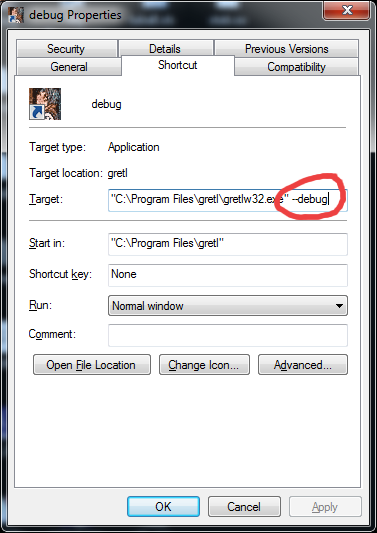
\includegraphics[scale=0.8]{figures/gretl-shortcut}
\end{figure}

When you start gretl in this mode, a ``console window'' appears as
well as the gretl window, and \texttt{stderr} output goes to the
console. To copy this output, click at the top left of the console
window for a menu (Figure~\ref{fig:gretl-debug}): first do ``Select
all'', then ``Copy.'' You can paste the results into Notepad or
similar.

\begin{figure}[htbp]
  \centering
  \caption{The program with console window}
  \label{fig:gretl-debug}
  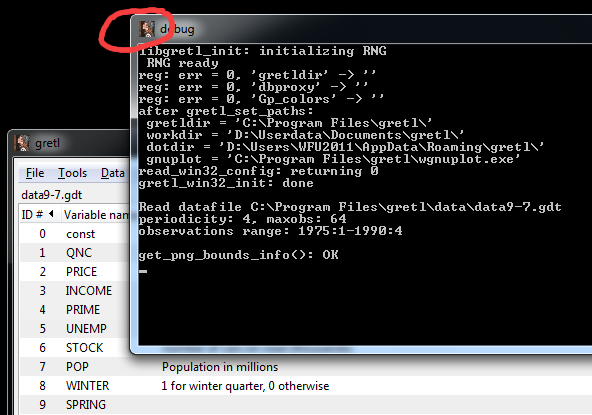
\includegraphics[scale=0.8]{figures/gretl-debug}
\end{figure}


\section{Auxiliary programs}
\label{trouble-programs}

As mentioned above, gretl calls some other programs to accomplish
certain tasks (gnuplot for graphing, {\LaTeX} for high-quality
typesetting of regression output, GNU R).  If something goes wrong
with such external links, it is not always easy for gretl to produce
an informative error message.  If such a link fails when accessed from
the gretl graphical interface, you may be able to get more information
by starting gretl from the command prompt rather than via a desktop
menu entry or icon.  On the X window system, start gretl from the
shell prompt in an \app{xterm}; on MS Windows, start the program
\cmd{gretl.exe} from a console window or ``DOS box'' using the
\verb|-g| or \option{debug} option flag.  Additional error messages
may be displayed on the terminal window.

Also please note that for most external calls, gretl assumes
that the programs in question are available in your ``path''---that
is, that they can be invoked simply via the name of the program,
without supplying the program's full location.\footnote{The exception
  to this rule is the invocation of gnuplot under MS Windows, where a
  full path to the program is given.}  Thus if a given program fails,
try the experiment of typing the program name at the command prompt,
as shown below.

\begin{center}
  \begin{tabular}{llll}
    & \textit{Graphing} & \textit{Typesetting} & \textit{GNU R}\\
    X window system & gnuplot & pdflatex & R\\
    MS Windows & wgnuplot.exe & pdflatex & RGui.exe\\
  \end{tabular}
\end{center}

If the program fails to start from the prompt, it's not a gretl issue
but rather that the program's home directory is not in your path, or
the program is not installed (properly).  For details on modifying
your path please see the documentation or online help for your
operating system or shell.
    
%%% Local Variables: 
%%% mode: latex
%%% TeX-master: "gretl-guide"
%%% End: 

